%!TEX program = xelatex
%\documentclass{cumcmthesis}
\documentclass[withoutpreface,bwprint]{cumcmthesis} %去掉封面与编号页，电子版提交的时候使用。
\usepackage[ruled, linesnumbered]{algorithm2e}
\usepackage[framemethod=TikZ]{mdframed}
\usepackage{url}   % 网页链接
\usepackage{subcaption} % 子标题
\usepackage{algorithmic} % 算法伪代码环境
\title{\textbf{泰迪杯}}
\tihao{A}
\schoolname{XX大学}
\membera{ }
\memberb{ }
\memberc{ }
\supervisor{ }
\yearinput{2020}
\monthinput{08}
\dayinput{22}

\begin{document}

\maketitle
\begin{abstract}
	本文针对两个连通教室内空气中示踪气体浓度的变化问题，基于物质守恒定律和流体混合原理，建立了双室耦合的微分方程动力学模型，并对空气混合过程及净化策略进行了深入研究。

	\textbf{针对问题一}，我们将两个教室视为两个通过空气交换相互作用的“隔室”，利用质量守恒定律建立了关于两个教室气体浓度随时间变化的\textbf{一阶线性常微分方程组}。模型考虑了教室容积差异及恒定的\textbf{交换流速}，能够准确描述浓度动态演变过程。

	\textbf{针对问题二}，通过解析求解上述微分方程组，我们得到了两个教室内气体浓度的显式时间函数。分析表明，系统最终将达到动态平衡。计算得出，两个教室的空气大约需要 \textbf{18至30分钟} 才能达到工程意义上的“混合均匀”（达到最终平衡值的95\%以上），最终两个教室的示踪气体浓度均将稳定在 \textbf{0.48 g/m³}。我们还为后勤部门撰写了通俗易懂的解释说明。

	\textbf{针对问题三}，为了实现教室B空气的快速净化，我们引入了与外部环境进行空气交换的控制变量，建立了含外部通风项的改进模型。通过对比不同通风速率下的\textbf{浓度衰减曲线}，论证了引入外部新风,如开窗通风或开启排气扇的必要性。仿真结果显示，增加对流至室外的通风量能显著破坏原有的封闭平衡，使污染物浓度呈指数级快速下降。

	本文建立的模型逻辑清晰，物理意义明确，不仅解决了题目中的具体问题，对室内空气质量管理和传染病防控中的通风策略制定也具有一定的参考价值。

	\keywords{\quad  微分方程模型\quad 物质守恒\quad 隔室模型\quad 动态平衡\quad 空气流通}
\end{abstract}

%目录  2019 明确不要目录，我觉得这个规定太好了
%\tableofcontents

%\newpage

\section{问题重述}

\subsection{问题背景}
随着资本市场信息披露透明度提升与投研分析需求高频化，传统基于人工拆解报表与静态BI工具的分析模式已难以满足跨周期、强关联的实时洞察需求，而直接调用大语言模型又面临资源冗余与时效不足的双重困境。为此，构建一套从自然语言输入到可视化分析结论输出的“智能问数”自动化链路，实现上市公司财报数据的零门槛、高效率查询与归因分析，成为提升投研决策精准度的关键突破口。

\subsection{问题提出}

为构建面向上市公司财报的零门槛智能分析系统，需依次解决以下三个核心问题：

任务一需从非结构化 PDF 财报中自动提取、校验并入库核心财务指标，构建完整规范的结构化数据库。

任务二需搭建具备意图识别、SQL数据库查询、多轮对话及数据可视化能力的智能助手，实现自然语言到分析结论的全流程自动化响应。

任务三需融合研报知识库，增强助手在多意图规划、输出校验与归因溯源方面的可靠性，确保分析结果可解释、可追溯。
\section{问题分析}

本课题旨在构建一套面向上市公司财报的“智能问数”自动化系统，涉及非结构化数据解析、自然语言处理与知识库增强检索三大核心环节。以下针对三个任务的具体难点与建模思路展开深入分析。

\subsection{任务一的分析：基于多源异构解析与勾稽校验的结构化建模}

任务一要求将非结构化PDF财报转化为规范的结构化表格并导入数据库。分析难点在
于上交所与深交所财报排版规则各异，表格字段对齐困难。为此，需设计鲁棒的表格
定位与字段映射算法，针对不同交易所的命名规则建立正则匹配模版，将数据准确写
入资产负债表、利润表、现金流量表及核心业绩指标表。此外，必须建立基于会计勾
稽关系的跨表校验模型（如 “资产总计 = 负债总计 + 所有者权益总计”），对异常波
动数据进行自动识别、合理截断，并标注异常原因，确保最终入库数据的准确性、完
整性与逻辑一致性。
\subsection{任务二的分析：基于意图识别与上下文关联的交互式查询建模}

任务二要求实现从自然语言到可视化结论的自动化响应。其核心在于构建“意图识别—
槽位填充—SQL查询”的映射模型。针对用户模糊提问，需建立基于关键要素熵值的主动
澄清引导机制；针对多轮对话场景，引入对话状态跟踪机制以维护上下文的公司实体
与时间窗口。在可视化环节，需建立图表类型匹配规则库（如时序数据对折线图、占比
数据对饼图），并结合统计描述模板自动生成数据结论，从而实现全流程的无人工干预
查询。

\subsection{任务三的分析：基于知识增强检索与任务自主规划的归因溯源建模}

任务三要求在结构化数据基础上融合个股与行业研报知识库以增强分析深度。首先
需对非结构化研报文本进行切片与向量索引构建，实现针对具体问题的相似段落召
回。针对多意图复合问题，需设计基于大语言模型的任务规划器，将复杂问句拆解
为有序的子任务序列集。最后，为增强结果可信度，需建立“数据—SQL—研
报摘要”的输出追溯链，在结果中明确标注引用来源与推理依据，实现从黑盒回答到
可解释归因分析的跃升。
\section{符号说明}
\begin{table}[H]
	\centering
	\begin{tabular}{ccc}
		\toprule[1.5pt]
		\makebox[0.3\textwidth][c]{变量名} & \makebox[0.4\textwidth][c]{符号说明} & \makebox[0.2\textwidth][c]{单位} \\
		\midrule[1pt]
		$T_tab$                         & 财报中的表格                           & $\text{m}^3$                   \\
		$T_text$                        & 财报中的文本                           & $\text{m}^3$                   \\
		$Q$                             & 教室间空气交换速率                        & $\text{m}^3/\text{min}$        \\
		$x(t)$                          & $t$时刻教室A中示踪气体的浓度                 & $\text{g/m}^3$                 \\
		$y(t)$                          & $t$时刻教室B中示踪气体的浓度                 & $\text{g/m}^3$                 \\
		$t$                             & 时间                               & $\text{min}$                   \\
		\bottomrule[1pt]
	\end{tabular}
\end{table}
\section{模型假设}

为了简化复杂的流体动力学过程，使模型具备可解性，同时保留问题的核心物理特征，本文提出以下基本假设：

\begin{enumerate}
	\item 假设教室 A、走廊和教室 B 均为理想的“完全混合箱室”。即污染物一旦进入某区域，瞬间与该区域内的空气均匀混合，浓度仅随时间变化，不随空间位置变化。
	\item 假设空气流动主要由压差或通风系统驱动，主导流向为“教室 A $\to$ 走廊 $\to$ 教室 B”以及“各区域 $\to$ 室外”。忽略微小的反向扩散（如从教室 B 逆流回走廊）。
	\item 假设各区域体积固定，且空气作为不可压缩流体，流入与流出的空气体积流量保持平衡（$Q_{in} = Q_{out}$）。
	\item 假设在模拟的时间段内，各房间的通风率、温度及扩散系数保持恒定，不随时间波动。
	\item 假设 $t=0$ 时刻，仅教室 A 存在初始污染物浓度 $C_0$，走廊和教室 B 的初始浓度均为 0。
\end{enumerate}
\newpage
\section{模型的建立与求解}
\subsection{任务一：非结构化财报数据的解析与数据库构建}
为确保上市公司财报数据的结构化存储与高效查询，本文设计并实现了一套端到端的自动化数据处理流水线，将非结构化PDF格式的财务报告转化为规范化的关系型数据库。该过程涵盖数据预处理、数据映射查找及计算、一致性校验三个核心环节。为后续智能助手平台搭建，我们构建了数据库，将解析得到的数据写入数据库。最终构建了包含核心业绩指标表、资产负债表、利润表及现金流量表四张核心表的财务数据库。\par

\subsubsection{非结构化财报数据的解析}
原始财务报告以 PDF 格式呈现，普遍存在版式复杂、表格与正文混排、关键数据跨页拆分等问题，难以直接用于结构化分析与建模。为此，本文先对报告进行解析将其从非结构化的pdf格式转换为可编辑的word格式，并从中精准提取财务表格，再经标准化数据清洗与规整处理，完成从非结构化财报到标准化结构化数据的转换。

（1）PDF格式转为Word格式

考虑到PDF文件在表格结构识别方面存在较大局限，我们引入Word作为中间载体，将PDF文档转换为可解析的Word格式。相比PDF，Word文档能够更清晰地保留表格边界、单元格结构及段落层级关系，从而为后续数据提取提供可靠基础。

\begin{table}[htbp]
	\centering
	\caption{PDF 与 WORD 对比}
	% 两列：左对齐 + 左对齐（可换成 c 居中）
	\begin{tabular}{cc}
		\toprule  % 顶线
		PDF                 & WORD              \\
		\midrule  % 中线
		适合扫描件与图像化表格,无内在行列结构 & 原生结构化强,自带行列标签     \\
		文本碎片化, 文字常被拆分为独立文本框 & 文本连续完整,便于直接复制使用   \\
		复杂排版兼容性差,易误判表格边界    & 合并单元格可识别,准确还原复杂表头 \\
		可编辑性差,提取后需大量人工整理    & 二次编辑成本极低,提取后可计算   \\
		\bottomrule % 底线
	\end{tabular}
\end{table}

财务报告形式上为报告类文字，非扫描件图片，转换可行性非常强。直接从pdf解析得到的表格，易出现列数错乱，数字与符号混乱，数据乱序等问题。我们借助 pdf2docx 将 PDF 精准还原为具备原生表格结构的 Word 文档，按版式还原并保留原生表格结构，使表格行列边界、单元格归属、文本对齐关系得到完整保留。

在此基础上再进行表格提取与数据清洗，能够显著提升表格结构还原度，避免因 PDF 非结构化渲染导致的数据错位、符号丢失与数值错乱，确保财务数据的完整性与准确性。


（2）表格抽取与上下文解析

在获得Word文档后，对其中的表格与段落进行统一解析。针对财务报表中“表格—标题—单位说明”紧密关联的特点，本文采用\textbf{上下文感知的表格抽取策略}，同时获取以下信息：

\begin{itemize}
	\item 表格内容（数值数据）
	\item 表格标题（用于识别报表类型）
	\item 单位信息（用于后续标准化）
	\item 页码与位置关系（用于跨页识别）
\end{itemize}

\textbf{上下文感知的表格抽取策略}是指在表格提取时，我们不只是简单将具备行列框架特征的表格进行提取，同时按 Word 文档自上而下的原始阅读顺序，依次提取段落与表格对象，构建连续的文档元素流，严格保留财务报表 “标题 — 单位 — 表格” 的空间邻近关系。在遍历文档流过程中，当识别到 “单位：万元”“合并资产负债表” 等财务关键段落时，立即缓存为上下文状态，当后续相邻表格出现时，自动将标题与单位绑定至该表格，实现 “上下文→表格” 的精准关联。

（3）跨页表格合并与报表筛选

针对财务报告中常见的跨页表格问题，我们利用分页上下文实现跨页表格的延续性判断与合并，有效解决财务报表因分页导致的表格断裂问题。在依次提取文档中表格及其上下文信息后，通过相邻页码判断、列数一致性校验、表格标题语义匹配、表头行相似性对比四项约束条件，判断后续表格是否为前一表格在分页后的延续。若满足延续条件，则剔除跨页位置重复出现的表头行，将多张分段表格的数据行进行纵向拼接，恢复为完整的单张财务报表结构，避免数据断裂与结构碎片化。

此外，由于原始报告中可能同时包含母公司报表与合并报表，本文基于关键词与语义规则进行筛选，优先保留合并财务报表，以保证数据口径一致性。

（4）单位统一与数据规范化

不同企业财报中常使用“元、千元、万元、亿元”等不同计量单位。为保证数据可比性，定义统一转换函数：

\begin{equation}
	x^{*} = \lambda \cdot x
\end{equation}

其中，$\lambda$ 为单位转换系数，$x^{*}$ 为标准化后的数值（单位统一为“元”）。

同时，对表格数据进行规范化处理，包括：1.千分位符号去除、2.括号负数转换（如“(100)”$\rightarrow$-100）、3.百分比数值还原\textbf{可以展示一个处理后的表格}

（5）预处理结果构建

经过上述处理，最终得到完整且数据单位统一的结构化合并报表集合：

\begin{equation}
	\mathcal{T}_{clean} = \{\text{合并资产负债表}, \text{合并利润表}，\text{合并所有者权益变动表}, \text{合并现金流量表}\}
\end{equation}


\paragraph{数据映射与计算}
针对非结构化财务报告中目标字段分布的结构差异特性，本文构建了结构优先的分
级数据映射机制，实现目标字段从结构化表格与非结构化文本中的精准定位与数值
提取。设目标字段集合为 $\mathcal{F}=\{f_1,f_2,\dots,f_n\}$，原始数据源
划分为结构化表格集合 $\mathcal{T}_{tab}$（财报中标准化表格）与非结构化文本集合 $\mathcal{T}_{text}$（Word 格式下财报全文）。

映射函数 $\mathcal{M}$ 遵循 由强结构到弱结构 的优先级原则，设计四层瀑布流提取策略
（表格优先映射层→文本上下文检索层→字段拓展匹配层→指标计算模型），逐层降低检索约束强度、拓展匹配维度
，既保证结构化数据的提取精度，又提升非结构化文本中字段的召回率，整体流程如图 1 所示：



（1）\textbf{表格优先映射层}:该层为强约束检索层，优先从结构化程度最高的财务
报表 CSV 文件中完成字段定位，是整个提取机制的核心基础。
\begin{itemize}
	\item 财务术语标准化处理:构建金融领域专用的同义词映射表
	      ，覆盖关键指标（如每股净资产、营业总收入、净利润等），
	      每类指标关联其标准名称、简称、行业通用别称。对目标字段名称执行标
	      准化清洗，清洗规则包括移除括号内注释、单位后缀、增减幅标识等冗余信息
	      ，保留字段核心语义。\\
	\item 精确匹配检索:基于清洗后的标准字段名，在已完成结构化解析的财务表格
	      中执行精确匹配与包含匹配\\
	\item 表格结构化解析:针对财报CSV文件的异构格式问题，设计自适应解析策略(多编码兼容读取,表头年份自动识别,报表类型自动分类)
\end{itemize}
（2）\textbf{文本上下文检索层}:当表格层未匹配到目标字段时，进入文本层检索，从Word格式财报全文中基于上
下文语义定位数值：
\[
	f_i = \mathcal{M}_2(\mathcal{T}_{text} \mid \text{context})
\]
其中 context 表示关键词上下文语义区域，定义为目标字段关键词所在段落的前1段+当前段+后1段构成的文本窗口。

文本检索规则如下：
\begin{itemize}[leftmargin=*]
	\item 关键词清洗：移除字段名中的空格，生成紧凑关键词；
	\item 排除性过滤：构建排除关键词列表（母公司、联营企业、少数股东等），若上下文包含该类关键词，则跳过当前匹配结果（避免非合并报表数据干扰）；
	\item 数值提取：通过正则表达式提取上下文内的数值，支持千分位分隔、负数括号表示、百分比等常见财务数值格式。
\end{itemize}

在提取时，增加同义词拓展：

\begin{itemize}[leftmargin=*]
	\item 规则1：匹配``即：XXX''格式，提取括号内的别称；
	\item 规则2：匹配``亦称/又称/别名：XXX''格式，拆分多别名；
\end{itemize}
拓展后的同义词集合用于提升文本检索的覆盖率。

（3）\textbf{字段拓展匹配层}:若前两层均未匹配到结果，采用语义匹配完成字段拓展检索，解决字段名称表述差异导致的匹配失效问题。

在语义相似度计算上：采用余弦相似度度量目标字段与候选文本的语义关联度：

\[
	\text{sim}(q,t)=\frac{q\cdot t}{\|q\|\|t\|}
\]

其中$q$为目标字段名称的向量表示，$t$为财报候选文本的向量表示，$\text{sim}(q,t)\in[0,1]$，值越大表
示语义相似度越高。

在字段拓展的具体方法上，我们使用了\textbf{金融专用SBERT模型}。并选用DMetaSoul/sbert-chinese-qmc-finance-v1-distill模型完成文本向量化，该模型基于金融语料预训练，适配财务术语的语义特征：

\begin{itemize}[leftmargin=*]
	\item 预计算缓存：对所有表格字段名预计算向量并缓存，避免重复计算；
	\item 类别约束匹配：结合表格类型分类结果（如资产负债表），仅在同类别候选字段中执行语义匹配，
	      提升匹配精度；
	\item 阈值筛选：设置相似度阈值0.85，仅当最大相似度≥阈值时，返回对应的数值结果。
\end{itemize}

（4）指标计算模块
在计算公式上我们根据会计基础知识，进行如下规定：


而在公式计算上，为构建安全的公式解析引擎，支持abs等基础数学函数，我们执行如下流程：
\begin{itemize}[leftmargin=*]
	\item 公式预处理：移除公式前缀的等号（=），替换字段占位符为实际数值；
	\item 安全执行：禁用内置函数与危险操作，仅开放白名单函数；
	\item 校验机制：对同时支持直接提取与公式计算的字段，对比两种方式的结果（误差阈值 $10^{-6}$），完成数据校验。
\end{itemize}
\paragraph{一致性校验}

为确保数据在进入模型前具有良好的可靠性与逻辑一致性，本文设计了一套多维约束驱动的数据校验机制。

会计恒等式约束为：

\begin{equation}
	A \approx L + E
\end{equation}

容差范围为：

\begin{equation}
	|A - (L+E)| \leq \epsilon
\end{equation}

跨期一致性约束为：

\begin{equation}
	\left| \frac{x_t - x_{t-1}}{x_{t-1}} \right| \leq \delta
\end{equation}

\subsection{数据库搭建部分（后续接在问题一后面）}
为实现数据来源的全程可追溯与入库数据的唯一性，本文设计了一套基于批次管理机制的数据导入流水
线。该流水线不仅负责将解析后的Excel结构化数据持久化至MySQL，更通过严格的事务控制与元数据记
录，保障每一次数据变更均可审计、可回滚、可复现。

\paragraph{文件溯源与批次管理}
为实现文件溯源， 在文件导入启动时，系统会生成一个全局唯一的批次标识符\texttt{id}，并在
相应的审计表中插入一条记录。该记录包含以下关键元
数据字段：执行导入的用户标识、源Excel文件的完整路径与文件名、文件的SHA256哈希值、导入起始
时间戳以及初始状态。文件哈希值的引入确保了数据溯源时能够唯一锁定原
始文件版本，防止因文件重名或内容篡改导致的数据来源混淆。

\paragraph{基于联合主键的文件更新机制}
为杜绝同一家公司同一报告期数据的重复存储，数据库表设计时将\texttt{(股票代码, 报告日期)}定义为联合唯一约束。\par
在数据写入环节，我们没有使用传统的插入或直接替换语句，而是采用了「不存在则插入，存在则更新」的处理逻辑：当待写入的记录，其股票代码与报告期的组合在数据库中已经存在时，系统会自动转为更新操作，用最新解析的数据覆盖原有记录，同时保持标识不变。\par
这一设计有两个明显的优势：\par
1.保证了导入数据的唯一性：即使同一份文件被多次导入，也不会产生重复、冗余的数据；\par
2.保障了数据关联的完整性：避免了传统 “先删除再插入” 的替换方式，可能引发的数据关联失效问题。

\paragraph{异常回滚}
在任意环节发生异常（如字段类型不匹配、网络中断等），事务将整体回滚，同时批次表的状态被更新为
\texttt{failed}并记录完整的异常堆栈信息。通过该设计确保了数据库不会写入残留的脏数据，
维持了数据的全局一致性。

\paragraph{数据的可视化追溯}系统为每一条财务数据记录配置了唯一\texttt{id}字段，实现了数据全生命周期的可追溯管理。通过关联数据导入批次信息，可对任意一条财务记录的来源与变更过程进行完整溯源，具体支持以下追溯场景：（如记录来源于哪个Excel文件，数据执行导入的操作者是谁等）
\subsection{任务二：面向财报的“智能询问”助手构建}
在任务一所构建的结构化财报数据库基础之上，本文设计并实现了一款面向上市公司财务数据的“智能问数”助手系统。
该系统遵循“自然语言输入→意图识别→SQL生成→数据查询→可视化呈现→分析结论输出”的全链路自动化架构，具备单轮基础查询、多轮上下文对话、
意图澄清引导及动态图表生成四项核心能力，最终以结构化JSON格式输出响应内容。
\begin{figure}[H]
	\centering
	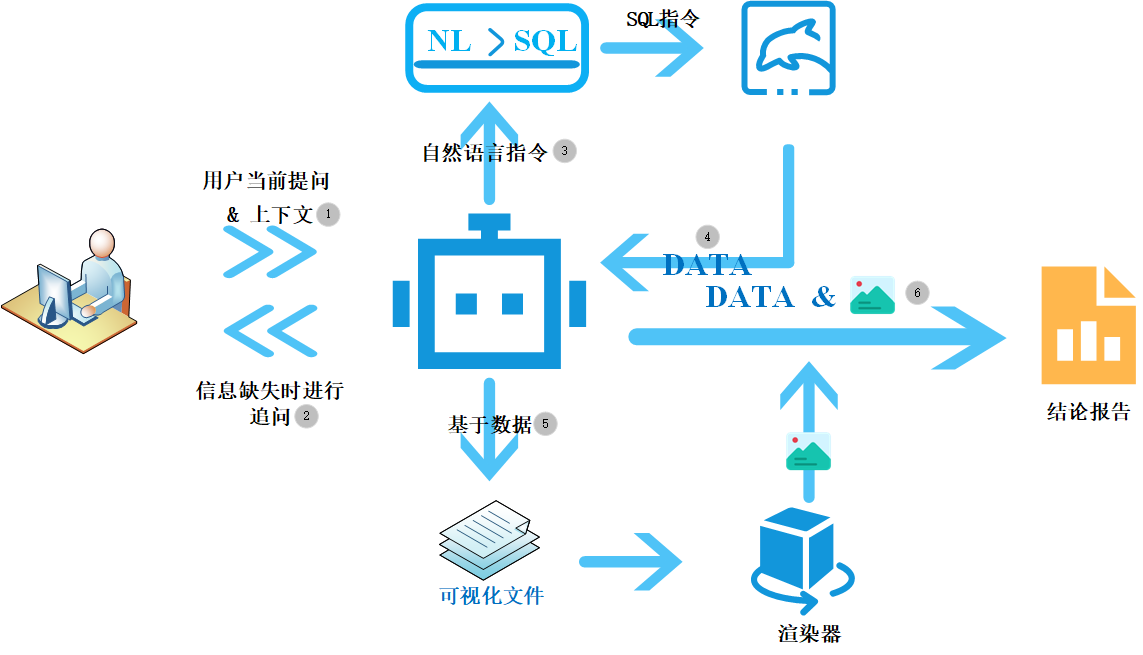
\includegraphics[width=0.90\textwidth]{2.png}
	\caption{智能询问助手系统架构图}
	\label{fig:单图}
\end{figure}
\subsubsection{系统总体架构}
针对任务二，为使系统职责清晰、模块化程度高，本文采取了分层设计。将智能询问助手系统拆解成四个协作层：
\begin{enumerate}
	\item \textbf{交互层}：接收用户输入并以流式方式实时回传状态与答案；
	\item \textbf{理解层}：完成意图识别、上下文继承与澄清决策；
	\item \textbf{执行层}：NL2SQL生成、安全校验、数据库查询；
	\item \textbf{表达层}：自动图表生成、文字结论组织、JSON结构化输出。
\end{enumerate}
\begin{figure}[H]
	\centering
	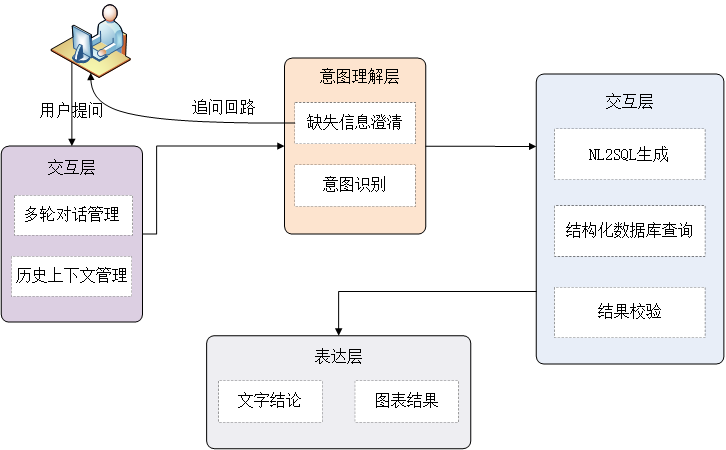
\includegraphics[width=0.90\textwidth]{3.png}
	\caption{询问助手协作层结构图}
	\label{fig:协作层结构图}
\end{figure}
\subsubsection{多轮对话与澄清机制}
智能助手并不是简单保留聊天记录，而是维护可执行查询所需的\textbf{状态变量}。系统维护的核心状态包括公司实体、报告期窗口、指标口径与上一轮查询结
果摘要。对于追问类问题，系统优先复用上一轮状态，只更新添加状态变量。通过状态变量的设置让系统能理解上下文语境，处理用户的追问，提高用户的交互效率与体验。

针对用户输入关键信息缺失或意图模糊时，系统触发澄清模块。澄清模块采用“模板保底+LLM增强”的混合策略：
\begin{enumerate}
	\item 首轮优先使用模板追问；
	\item 在用户模糊回答或复杂场景下调用LLM二次追问；
	\item 信息满足执行条件后自动进入NL2SQL流程。
\end{enumerate}
通过该策略在评测中有效减少了“错误SQL”和“答非所问”现象。
\begin{figure}[H]
	\centering
	
\includegraphics[width=0.90\textwidth]{1.png}
	\caption{澄清策略前后效果对比}
\end{figure}
\subsubsection{基于大语言模型的NL2SQL生成引擎}
本模块旨在将用户自然语言查询自动转化为可执行的结构化查询语句，并在数据库内容基础上生成可解释的分析结论。
其核心逻辑为先让大语言模型完成“语义理解与查询规划”，再由数据库返回事实数据，最后由大语言模型负责归纳与解释，
从而避免数据伪造提高结果的可核验性。\par
从形式化角度，给定用户问题 $q$、数据库模式信息 $S$与对话上下文 $C$，NL2SQL 任务可表示为：
\[
	\hat{s} = \arg\max_{s \in \mathcal{S}} P(s \mid q, S, C; \theta),
\]\par
其中 $\hat{s}$ 为生成的 SQL，$\theta$ 为大语言模型参数。查询执行后得到结果集 $R = \text{Exec}(\hat{s})$，最终分析结论为：
\[
	\hat{a} = G(q, R, C),
\]\par
其中 $G(\cdot)$ 表示基于结构化结果的分析生成函数。\par

\begin{algorithm}[htbp]
	\caption{NL2SQL 生成与执行主流程}
	\SetKwInOut{Input}{输入}
	\SetKwInOut{Output}{输出}
	\SetInd{0.5em}{1em} % 调整缩进间距

	\Input{用户问题 $q$, 对话上下文 $C$, 数据库模式 $S$, 表白名单 $T_{allow}$}
	\Output{回答 $A$, 元信息 $M$}
	\BlankLine % 中间的分隔线（类似 midrule 效果）

	% 步骤1：意图识别
	\If{$\neg \text{IsFinanceQuery}(q)$}{
		\Return $\text{GeneralLLMAnswer}(q, C), \emptyset$\;
	}

	% 步骤2：JSON 生成与解析
	$P \leftarrow \text{BuildPrompt}(q, C, S)$\;
	$J \leftarrow \text{LLM\_Generate\_JSON}(P)$\;

	\If{$\text{ParseFailed}(J) \lor \neg J.\text{need\_sql}$}{
		\Return $\text{GeneralLLMAnswer}(q, C), \emptyset$\;
	}

	% 步骤3：SQL 安全校验
	$sql \leftarrow J.\text{sql}$\;
	\If{$\neg \text{IsSafeSelect}(sql, T_{allow})$}{
		\Return $\text{SafeFallbackAnswer}(q), \{\text{reason: ``unsafe''}\}$\;
	}

	% 步骤4：数据执行与元信息构建
	$R \leftarrow \text{ExecSQLWithLimit}(sql, L_{max})$\;
	$M \leftarrow \{ \text{sql}: sql, \text{count}: |R|, \text{cols}: \text{Cols}(R), \text{data}: \text{Head}(R, k) \}$\;

	% 步骤5：结果生成
	$K \leftarrow \text{BuildResultContext}(M, R)$\;
	$A \leftarrow \text{StreamAnalysisAnswer}(q, C, K)$\;

	\Return $(A, M)$\;
\end{algorithm}

\subsubsection{自动图表生成与证据化表达}
为满足“可视化输出”要求，系统在SQL结果返回后自动进行图表规划。不同于直接让模型执行任意代码，本文采用“\textbf{模型决策+固定渲染器执行}”方案：
\begin{enumerate}
	\item 大语言模型根据结果字段与问题语义给出图表规格（如折线/柱状/饼图）；
	\item 后端受控渲染器执行绘图并将图片保存到\texttt{result}目录下；
	\item 在流式回复中实时告知图片文件名与保存路径，并结合图表给出结论分析解释。
\end{enumerate}
\subsubsection{流式交互与最终输出结构}
在用户体验层，系统采用事件驱动流式输出。每轮交互会按阶段返回状态：意图分析、SQL生成、SQL执行、图表生成、结论生成。用户可以通过后端的可视化界面，看到系统
“正在做什么”。

最终输出与要求格式保持一致：
\begin{equation}
	\text{Answer} = \{\text{content},\ \text{image},\ \text{references}\}
\end{equation}
其中\texttt{image}为自动生成图表的相对路径列表，\texttt{content}为结合数据证据的分析结论。
\subsubsection{模型展示与结果输出}
\section{灵敏度分析 }
\section{模型评价 }

\subsection{模型的优点}
\begin{enumerate}
	\item 模型基于物质守恒定律和流体混合原理，具有坚实的物理基础，能够准确描述两个教室内示踪气体浓度随时间的动态演变过程。
\end{enumerate}

\subsection{模型的缺点与改进}
\begin{enumerate}
	\item “均匀混合”假设的局限性：模型假设教室内空气瞬间均匀混合，忽略了污染物在房间角落或远离门窗区域的空间分布差异。在实际大空间教室中，可能存在局部浓度过高的死角。
\end{enumerate}

% =============================================================
% 参考文献
% =============================================================

\begin{thebibliography}{99}

	\bibitem{jiang2011}
	姜启源, 谢金星, 叶俊. \textit{数学建模 (第4版)}. 北京: 高等教育出版社, 2011.


\end{thebibliography}


\newpage
%附录
\begin{appendices}

	\newpage
	\section{附录：主要Python求解代码}

	\subsection{问题二：双教室气体交换动力学模拟}
	\label{code:prob1}

	\begin{lstlisting}[caption={问题一浓度变化模拟代码}, label={lst:code1}]
	import numpy as np
	import matplotlib.pyplot as plt
	from scipy.integrate import odeint
	
	# 1. 参数设置
	V_A = 150.0  # 教室A体积 (m^3)
	V_B = 100.0  # 教室B体积 (m^3)
	Q = 10.0     # 交换速率 (m^3/min)
	C_A_init = 0.8
	C_B_init = 0.0
	
	# 2. 定义微分方程组
	def exchange_model(C, t):
	C_A, C_B = C
	dC_A_dt = (Q * C_B - Q * C_A) / V_A
	dC_B_dt = (Q * C_A - Q * C_B) / V_B
	return [dC_A_dt, dC_B_dt]
	
	# 3. 求解
	t = np.linspace(0, 60, 1000)
	sol = odeint(exchange_model, [C_A_init, C_B_init], t)
	
	# 4. 绘图 (省略部分格式化代码)
	plt.plot(t, sol[:, 0], label='Classroom A')
	plt.plot(t, sol[:, 1], label='Classroom B')
	plt.axhline(y=0.48, color='green', linestyle='--', label='Equilibrium (0.48)')
	plt.legend()
	plt.show()
\end{lstlisting}

	\subsection{问题三：不同净化策略的对比分析}
	\label{code:prob3}

	该脚本用于对比“基准策略”、“仅通风策略”与“隔离+通风策略”的效果。

	\begin{lstlisting}[caption={问题三净化策略对比仿真代码}, label={lst:code3}]
	import numpy as np
	import matplotlib.pyplot as plt
	from scipy.integrate import odeint
	
	# 参数定义
	V_A, V_B = 150.0, 100.0
	C_A0, C_B0 = 0.8, 0.0
	
	def strategy_model(C, t, Q_door, Q_vent):
	"""
	Q_door: 教室间交换率 (关门=0)
	Q_vent: 教室B排风率
	"""
	C_A, C_B = C
	dC_A_dt = (Q_door * C_B - Q_door * C_A) / V_A
	dC_B_dt = (Q_door * C_A - Q_door * C_B - Q_vent * C_B) / V_B
	return [dC_A_dt, dC_B_dt]
	
	t = np.linspace(0, 30, 600)
	init_C = [C_A0, C_B0]
	
	# 策略1: 基准 (开门, 无排风)
	sol1 = odeint(strategy_model, init_C, t, args=(10.0, 0.0))
	
	# 策略2: 仅通风 (开门, 排风20)
	sol2 = odeint(strategy_model, init_C, t, args=(10.0, 20.0))
	
	# 策略3: 隔离+通风 (关门, 排风20)
	sol3 = odeint(strategy_model, init_C, t, args=(0.0, 20.0))
	
	# 绘图部分
	plt.plot(t, sol1[:, 1], label='Strategy 1: Baseline')
	plt.plot(t, sol2[:, 1], label='Strategy 2: Vent Only')
	plt.plot(t, sol3[:, 1], label='Strategy 3: Isolation+Vent')
	plt.axhline(y=0.05, color='r', linestyle=':', label='Threshold')
	plt.legend()
	plt.show()
\end{lstlisting}

	\subsection{灵敏度分析代码}
	\label{code:sensitivity}

	用于分析走廊/门洞交换速率的不确定性对混合时间的影响。

	\begin{lstlisting}[caption={参数灵敏度分析代码}, label={lst:code_sens}]
	# 定义灵敏度分析函数
	def get_mixing_time(Q_val):
	# 求解特定Q下的方程
	sol = odeint(exchange_model_modified, init_C, t, args=(Q_val,))
	C_B = sol[:, 1]
	# 查找达到0.4的时间索引
	idx = np.where(C_B >= 0.4)[0]
	if len(idx) > 0:
	return t[idx[0]]
	else:
	return np.nan
	
	# 设定波动范围 (-20% to +20%)
	variations = [0.8, 0.9, 1.0, 1.1, 1.2]
	base_Q = 10.0
	
	print("Sensitivity Analysis Results:")
	print("Variation | Q Value | Mixing Time | Time Change")
	for v in variations:
	Q_new = base_Q * v
	t_mix = get_mixing_time(Q_new)
	print(f"{v-1:.0%} | {Q_new:.1f} | {t_mix:.2f} min")

	\end{lstlisting}
\end{appendices}

\end{document}